% =============================================================================
% Model Architecture: Adversarial Disentanglement for Audio Deepfake Detection
% LaTeX Document for Research Paper Inclusion
% =============================================================================

\documentclass[11pt]{article}
\usepackage[utf8]{inputenc}
\usepackage{amsmath,amssymb,amsfonts}
\usepackage{graphicx}
\usepackage{booktabs}
\usepackage{multirow}
\usepackage{algorithm}
\usepackage{algpseudocode}
\usepackage{tikz}
\usetikzlibrary{shapes,arrows,positioning,fit,backgrounds}
\usepackage{xcolor}
\usepackage{hyperref}

% Custom colors
\definecolor{prosodyblue}{RGB}{227,242,253}
\definecolor{contentorange}{RGB}{255,243,224}
\definecolor{discrimred}{RGB}{252,228,236}
\definecolor{lossgreen}{RGB}{232,245,233}

\begin{document}

% =============================================================================
\section{Proposed Architecture}
% =============================================================================

We propose an adversarial disentanglement framework for audio deepfake detection that explicitly separates prosodic features from linguistic content. The architecture consists of three interconnected components: (1) a Prosody Encoder that extracts spoofing-relevant features from mel-spectrograms, (2) a frozen Content Encoder based on Wav2Vec 2.0 that captures linguistic representations, and (3) a Content Discriminator with gradient reversal that enforces content-invariant feature learning.

% =============================================================================
\subsection{System Overview}
% =============================================================================

Let $\mathbf{x} \in \mathbb{R}^{T}$ denote a raw audio waveform of duration $T$ samples. Our framework processes this input through two parallel pathways:

\begin{enumerate}
    \item \textbf{Prosodic Pathway}: $\mathbf{x} \xrightarrow{\text{MelSpec}} \mathbf{M} \xrightarrow{f_\theta} (\mathbf{z}_p, \hat{y})$
    \item \textbf{Content Pathway}: $\mathbf{x} \xrightarrow{g_\phi} \mathbf{z}_c$
\end{enumerate}

where $\mathbf{M} \in \mathbb{R}^{F \times T'}$ is the mel-spectrogram with $F$ mel bins and $T'$ time frames, $f_\theta$ is the trainable Prosody Encoder parameterized by $\theta$, $g_\phi$ is the frozen Wav2Vec 2.0 Content Encoder with pre-trained parameters $\phi$, $\mathbf{z}_p \in \mathbb{R}^{d_p}$ are the prosody features, $\mathbf{z}_c \in \mathbb{R}^{d_c}$ are the content features, and $\hat{y} \in \{0, 1\}$ is the spoofing prediction.

% =============================================================================
\subsection{Input Preprocessing}
% =============================================================================

Raw audio waveforms are first converted to mel-spectrogram representations using the following parameters:

\begin{table}[h]
\centering
\caption{Mel-spectrogram extraction parameters}
\label{tab:mel_params}
\begin{tabular}{@{}lcc@{}}
\toprule
\textbf{Parameter} & \textbf{Value} & \textbf{Description} \\
\midrule
Sample Rate & 16,000 Hz & Standard for speech \\
Duration & 4 seconds & Maximum audio length \\
N\_FFT & 400 & 25ms window \\
Hop Length & 160 & 10ms stride \\
Mel Bins ($F$) & 80 & Frequency resolution \\
Time Frames ($T'$) & 401 & Temporal resolution \\
\bottomrule
\end{tabular}
\end{table}

The mel-spectrogram is computed as:
\begin{equation}
    \mathbf{M}_{f,t} = \sum_{k=0}^{N-1} W_f(k) \cdot |\text{STFT}(\mathbf{x})_{k,t}|^2
\end{equation}
where $W_f(k)$ denotes the $f$-th mel filterbank weight at frequency bin $k$.

% =============================================================================
\subsection{Prosody Encoder}
% =============================================================================

The Prosody Encoder $f_\theta: \mathbb{R}^{1 \times F \times T'} \rightarrow (\mathbb{R}^{d_p}, \mathbb{R}^{2})$ is a ResNet-inspired convolutional neural network designed to capture temporal prosodic patterns from mel-spectrograms.

\subsubsection{Residual Block}

Each residual block follows the pre-activation design:
\begin{equation}
    \mathbf{h}_{l+1} = \sigma\Big(\mathcal{F}(\mathbf{h}_l; \mathbf{W}_l) + \mathcal{S}(\mathbf{h}_l)\Big)
\end{equation}
where $\mathcal{F}$ represents the residual mapping consisting of two convolutional layers:
\begin{equation}
    \mathcal{F}(\mathbf{h}; \mathbf{W}) = \text{BN}\Big(\text{Conv}_{3\times3}\big(\sigma(\text{BN}(\text{Conv}_{3\times3}(\mathbf{h})))\big)\Big)
\end{equation}
and $\mathcal{S}$ is the shortcut connection:
\begin{equation}
    \mathcal{S}(\mathbf{h}) = 
    \begin{cases}
        \mathbf{h} & \text{if } C_{in} = C_{out} \text{ and } s = 1 \\
        \text{Conv}_{1\times1}(\mathbf{h}) & \text{otherwise}
    \end{cases}
\end{equation}

\subsubsection{Network Architecture}

The complete Prosody Encoder architecture is summarized in Table~\ref{tab:prosody_arch}.

\begin{table}[h]
\centering
\caption{Prosody Encoder layer specifications}
\label{tab:prosody_arch}
\begin{tabular}{@{}lcccr@{}}
\toprule
\textbf{Layer} & \textbf{Input} & \textbf{Output} & \textbf{Stride} & \textbf{Params} \\
\midrule
Conv1 + BN & $(1, 80, 401)$ & $(64, 80, 401)$ & $1$ & 640 \\
ResBlock$_1$ & $(64, 80, 401)$ & $(64, 80, 201)$ & $(1, 2)$ & 73,856 \\
ResBlock$_2$ & $(64, 80, 201)$ & $(128, 40, 101)$ & $(2, 2)$ & 221,440 \\
ResBlock$_3$ & $(128, 40, 101)$ & $(256, 20, 51)$ & $(2, 2)$ & 885,248 \\
ResBlock$_4$ & $(256, 20, 51)$ & $(512, 10, 26)$ & $(2, 2)$ & 3,539,968 \\
AvgPool & $(512, 10, 26)$ & $(512, 1, 1)$ & — & 0 \\
FC$_1$ & $512$ & $256$ & — & 131,328 \\
FC$_2$ & $256$ & $2$ & — & 514 \\
\midrule
\textbf{Total} & — & — & — & \textbf{4,852,994} \\
\bottomrule
\end{tabular}
\end{table}

The forward pass can be expressed as:
\begin{align}
    \mathbf{h}_0 &= \sigma\big(\text{BN}(\text{Conv}_{3\times3}(\mathbf{M}))\big) \\
    \mathbf{h}_l &= \text{ResBlock}_l(\mathbf{h}_{l-1}), \quad l \in \{1, 2, 3, 4\} \\
    \mathbf{v} &= \text{AvgPool}(\mathbf{h}_4) \in \mathbb{R}^{512} \\
    \mathbf{z}_p &= \sigma(\mathbf{W}_1 \mathbf{v} + \mathbf{b}_1) \in \mathbb{R}^{256} \\
    \hat{\mathbf{y}} &= \mathbf{W}_2 \mathbf{z}_p + \mathbf{b}_2 \in \mathbb{R}^{2}
\end{align}
where $\sigma$ denotes the ReLU activation function.

% =============================================================================
\subsection{Content Encoder}
% =============================================================================

The Content Encoder $g_\phi: \mathbb{R}^{T} \rightarrow \mathbb{R}^{d_c}$ employs a pre-trained Wav2Vec 2.0 Base model \cite{baevski2020wav2vec} to extract semantic content representations. All parameters $\phi$ remain frozen during training.

\begin{table}[h]
\centering
\caption{Wav2Vec 2.0 Base specifications}
\label{tab:wav2vec}
\begin{tabular}{@{}ll@{}}
\toprule
\textbf{Property} & \textbf{Value} \\
\midrule
Architecture & 12-layer Transformer \\
Hidden Dimension ($d_c$) & 768 \\
Attention Heads & 12 \\
Parameters & 94.4M (frozen) \\
Pre-training Data & LibriSpeech 960h \\
\bottomrule
\end{tabular}
\end{table}

The content features are computed via temporal mean pooling:
\begin{equation}
    \mathbf{z}_c = \frac{1}{T''} \sum_{t=1}^{T''} \mathbf{h}_t^{(L)}
\end{equation}
where $\mathbf{h}_t^{(L)} \in \mathbb{R}^{768}$ is the hidden state at time step $t$ from the final transformer layer $L$, and $T''$ is the number of output frames.

% =============================================================================
\subsection{Adversarial Content Discriminator}
% =============================================================================

The Content Discriminator $D_\psi: \mathbb{R}^{d_p} \rightarrow \mathbb{R}^{d_c}$ attempts to reconstruct content features from prosody features. Crucially, it incorporates a Gradient Reversal Layer (GRL) \cite{ganin2015unsupervised} to enforce content-invariant representation learning.

\subsubsection{Gradient Reversal Layer}

The GRL is defined as an identity function during forward propagation with negated gradients during backpropagation:
\begin{align}
    \text{Forward:} \quad &\text{GRL}_\lambda(\mathbf{z}) = \mathbf{z} \\
    \text{Backward:} \quad &\frac{\partial \mathcal{L}}{\partial \mathbf{z}} \leftarrow -\lambda \cdot \frac{\partial \mathcal{L}}{\partial \text{GRL}_\lambda(\mathbf{z})}
\end{align}
where $\lambda \geq 0$ controls the strength of the gradient reversal.

\subsubsection{Discriminator Architecture}

The discriminator consists of a two-layer MLP:
\begin{align}
    \tilde{\mathbf{z}}_p &= \text{GRL}_\lambda(\mathbf{z}_p) \\
    \mathbf{h}_d &= \sigma(\mathbf{W}_3 \tilde{\mathbf{z}}_p + \mathbf{b}_3) \in \mathbb{R}^{256} \\
    \hat{\mathbf{z}}_c &= \mathbf{W}_4 \mathbf{h}_d + \mathbf{b}_4 \in \mathbb{R}^{768}
\end{align}

% =============================================================================
\subsection{Training Objective}
% =============================================================================

The overall training objective combines spoofing detection with adversarial content prediction:
\begin{equation}
    \mathcal{L}_{\text{total}} = \mathcal{L}_{\text{spoof}} + \lambda_{\text{adv}} \cdot \mathcal{L}_{\text{adv}}
\end{equation}

\subsubsection{Spoofing Detection Loss}

The primary classification task uses cross-entropy loss:
\begin{equation}
    \mathcal{L}_{\text{spoof}} = -\frac{1}{N} \sum_{i=1}^{N} \left[ y_i \log(\hat{p}_i^{(1)}) + (1 - y_i) \log(\hat{p}_i^{(0)}) \right]
\end{equation}
where $\hat{p}_i = \text{softmax}(\hat{\mathbf{y}}_i)$ and $y_i \in \{0, 1\}$ is the ground truth label (0: bonafide, 1: spoof).

\subsubsection{Adversarial Content Loss}

The adversarial objective minimizes content reconstruction error:
\begin{equation}
    \mathcal{L}_{\text{adv}} = \frac{1}{N} \sum_{i=1}^{N} \|\hat{\mathbf{z}}_{c,i} - \mathbf{z}_{c,i}\|_2^2
\end{equation}

Due to the gradient reversal, minimizing $\mathcal{L}_{\text{adv}}$ with respect to the discriminator parameters $\psi$ \emph{maximizes} it with respect to the encoder parameters $\theta$, encouraging the Prosody Encoder to learn features that cannot predict content.

\subsubsection{Adversarial Weight Scheduling}

The adversarial weight $\lambda_{\text{adv}}$ follows a warmup schedule:
\begin{equation}
    \lambda_{\text{adv}}(e) = 
    \begin{cases}
        0 & \text{if } e < e_{\text{warmup}} \\
        \lambda_{\text{base}} & \text{otherwise}
    \end{cases}
\end{equation}
where $e$ is the current epoch, $e_{\text{warmup}} = 5$, and $\lambda_{\text{base}} = 1.0$.

% =============================================================================
\subsection{Gradient Flow Analysis}
% =============================================================================

During backpropagation, the gradient flow through the system can be analyzed as follows. Let $\mathcal{L} = \mathcal{L}_{\text{spoof}} + \lambda_{\text{adv}} \mathcal{L}_{\text{adv}}$. The gradients with respect to the Prosody Encoder parameters $\theta$ are:

\begin{equation}
    \frac{\partial \mathcal{L}}{\partial \theta} = \underbrace{\frac{\partial \mathcal{L}_{\text{spoof}}}{\partial \theta}}_{\text{detection gradient}} - \lambda \cdot \lambda_{\text{adv}} \underbrace{\frac{\partial \mathcal{L}_{\text{adv}}}{\partial \theta}}_{\text{reversed content gradient}}
\end{equation}

The negative sign arises from the gradient reversal layer, creating an adversarial game where:
\begin{itemize}
    \item The \textbf{Prosody Encoder} tries to minimize $\mathcal{L}_{\text{spoof}}$ while maximizing $\mathcal{L}_{\text{adv}}$
    \item The \textbf{Discriminator} tries to minimize $\mathcal{L}_{\text{adv}}$
\end{itemize}

At equilibrium, the prosody features $\mathbf{z}_p$ become maximally informative for spoofing detection while being uninformative for content prediction.

% =============================================================================
\subsection{Implementation Details}
% =============================================================================

\begin{table}[h]
\centering
\caption{Training hyperparameters}
\label{tab:hyperparams}
\begin{tabular}{@{}ll@{}}
\toprule
\textbf{Hyperparameter} & \textbf{Value} \\
\midrule
Optimizer & Adam \\
Learning Rate & $1 \times 10^{-4}$ \\
Batch Size & 16 \\
Epochs & 50 \\
Steps per Epoch & 500 \\
Validation Steps & 100 \\
Gradient Clipping & 3.0 \\
Warmup Epochs & 5 \\
$\lambda_{\text{base}}$ & 1.0 \\
\bottomrule
\end{tabular}
\end{table}

% =============================================================================
\subsection{Theoretical Motivation}
% =============================================================================

The adversarial disentanglement framework is motivated by the hypothesis that \textit{spoofing artifacts primarily manifest in prosodic characteristics} (pitch patterns, rhythm, energy contours) rather than linguistic content. By explicitly forcing the Prosody Encoder to discard content information, we encourage the learning of:

\begin{enumerate}
    \item \textbf{Content-invariant features}: Representations that focus on prosodic anomalies universal across different texts and contexts
    \item \textbf{Speaker-independent patterns}: Features that generalize across diverse speaker characteristics
    \item \textbf{Attack-agnostic cues}: Artifacts common to multiple spoofing generation methods
\end{enumerate}

This approach draws inspiration from domain adaptation literature \cite{ganin2015unsupervised}, where gradient reversal has been successfully applied to learn domain-invariant representations for transfer learning.

% =============================================================================
% ALGORITHM BLOCK
% =============================================================================

\begin{algorithm}[h]
\caption{Adversarial Disentanglement Training}
\label{alg:training}
\begin{algorithmic}[1]
\Require Training data $\mathcal{D} = \{(\mathbf{x}_i, y_i)\}_{i=1}^N$
\Require Prosody Encoder $f_\theta$, Content Encoder $g_\phi$ (frozen), Discriminator $D_\psi$
\Require Learning rate $\eta$, adversarial weight $\lambda_{\text{base}}$, warmup epochs $e_w$
\For{epoch $e = 1$ to $E$}
    \State $\lambda_{\text{adv}} \gets \begin{cases} 0 & \text{if } e < e_w \\ \lambda_{\text{base}} & \text{otherwise} \end{cases}$
    \For{batch $(\mathbf{X}, \mathbf{y}) \in \mathcal{D}$}
        \State $\mathbf{M} \gets \text{MelSpectrogram}(\mathbf{X})$ \Comment{Extract mel-spectrograms}
        \State $\mathbf{Z}_p, \hat{\mathbf{Y}} \gets f_\theta(\mathbf{M})$ \Comment{Prosody features \& predictions}
        \State $\mathbf{Z}_c \gets g_\phi(\mathbf{X})$ \Comment{Content features (no grad)}
        \State $\hat{\mathbf{Z}}_c \gets D_\psi(\text{GRL}_\lambda(\mathbf{Z}_p))$ \Comment{Predicted content}
        \State $\mathcal{L}_{\text{spoof}} \gets \text{CrossEntropy}(\hat{\mathbf{Y}}, \mathbf{y})$
        \State $\mathcal{L}_{\text{adv}} \gets \text{MSE}(\hat{\mathbf{Z}}_c, \mathbf{Z}_c)$
        \State $\mathcal{L} \gets \mathcal{L}_{\text{spoof}} + \lambda_{\text{adv}} \cdot \mathcal{L}_{\text{adv}}$
        \State $\theta, \psi \gets \theta - \eta \nabla_\theta \mathcal{L}, \psi - \eta \nabla_\psi \mathcal{L}$
    \EndFor
    \State Evaluate on validation set and save best model
\EndFor
\end{algorithmic}
\end{algorithm}

% =============================================================================
% FIGURE: ARCHITECTURE DIAGRAM (TikZ)
% =============================================================================

\begin{figure}[h]
\centering
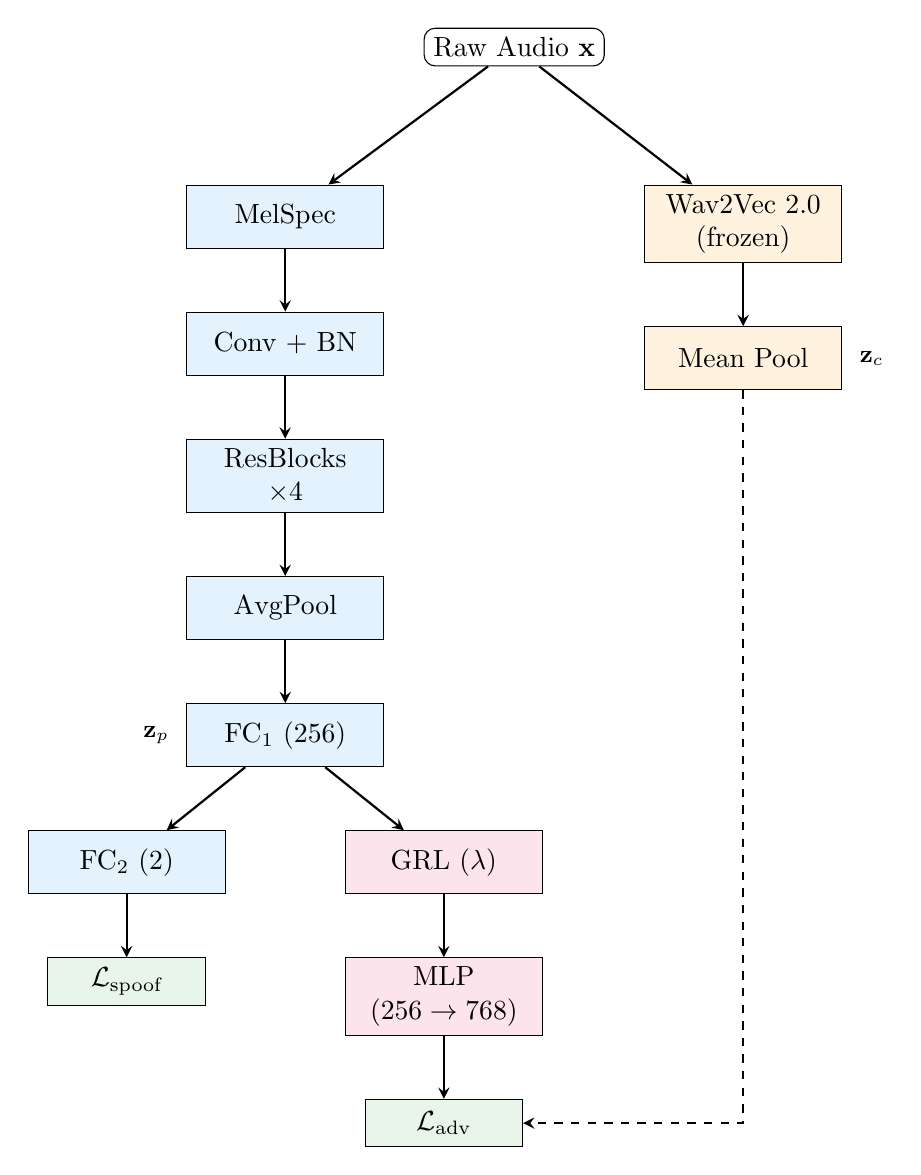
\begin{tikzpicture}[
    node distance=1.5cm,
    block/.style={rectangle, draw, fill=prosodyblue, minimum width=2.5cm, minimum height=0.8cm, align=center},
    blockc/.style={rectangle, draw, fill=contentorange, minimum width=2.5cm, minimum height=0.8cm, align=center},
    blockd/.style={rectangle, draw, fill=discrimred, minimum width=2.5cm, minimum height=0.8cm, align=center},
    blockg/.style={rectangle, draw, fill=lossgreen, minimum width=2cm, minimum height=0.6cm, align=center},
    arrow/.style={->, >=stealth, thick}
]

% Input
\node[draw, rounded corners] (audio) {Raw Audio $\mathbf{x}$};

% Prosody Encoder Branch
\node[block, below left=1.5cm and 0.5cm of audio] (mel) {MelSpec};
\node[block, below=0.8cm of mel] (conv) {Conv + BN};
\node[block, below=0.8cm of conv] (res) {ResBlocks\\$\times 4$};
\node[block, below=0.8cm of res] (pool) {AvgPool};
\node[block, below=0.8cm of pool] (fc1) {FC$_1$ (256)};
\node[block, below left=0.8cm and -0.5cm of fc1] (fc2) {FC$_2$ (2)};

% Content Encoder Branch
\node[blockc, below right=1.5cm and 0.5cm of audio] (w2v) {Wav2Vec 2.0\\(frozen)};
\node[blockc, below=0.8cm of w2v] (meanpool) {Mean Pool};

% Discriminator Branch
\node[blockd, below right=0.8cm and -0.5cm of fc1] (grl) {GRL ($\lambda$)};
\node[blockd, below=0.8cm of grl] (mlp) {MLP\\$(256 \to 768)$};

% Loss nodes
\node[blockg, below=0.8cm of fc2] (lspoof) {$\mathcal{L}_{\text{spoof}}$};
\node[blockg, below=0.8cm of mlp] (ladv) {$\mathcal{L}_{\text{adv}}$};

% Arrows - Prosody path
\draw[arrow] (audio) -- (mel);
\draw[arrow] (mel) -- (conv);
\draw[arrow] (conv) -- (res);
\draw[arrow] (res) -- (pool);
\draw[arrow] (pool) -- (fc1);
\draw[arrow] (fc1) -- (fc2);
\draw[arrow] (fc2) -- (lspoof);

% Arrows - Content path
\draw[arrow] (audio) -- (w2v);
\draw[arrow] (w2v) -- (meanpool);

% Arrows - Discriminator path
\draw[arrow] (fc1) -- (grl);
\draw[arrow] (grl) -- (mlp);
\draw[arrow] (mlp) -- (ladv);
\draw[arrow, dashed] (meanpool) |- (ladv);

% Labels
\node[left=0.1cm of fc1, font=\small] {$\mathbf{z}_p$};
\node[right=0.1cm of meanpool, font=\small] {$\mathbf{z}_c$};

\end{tikzpicture}
\caption{Proposed adversarial disentanglement architecture. The Prosody Encoder (blue) extracts features from mel-spectrograms for spoofing detection. The frozen Content Encoder (orange) provides content supervision. The Content Discriminator (red) with gradient reversal enforces content-invariant learning.}
\label{fig:architecture}
\end{figure}

% =============================================================================
% REFERENCES (Example - adjust to your paper's format)
% =============================================================================

\begin{thebibliography}{9}

\bibitem{ganin2015unsupervised}
Ganin, Y., \& Lempitsky, V. (2015).
\textit{Unsupervised Domain Adaptation by Backpropagation}.
In International Conference on Machine Learning (ICML).

\bibitem{baevski2020wav2vec}
Baevski, A., Zhou, H., Mohamed, A., \& Auli, M. (2020).
\textit{wav2vec 2.0: A Framework for Self-Supervised Learning of Speech Representations}.
In Advances in Neural Information Processing Systems (NeurIPS).

\bibitem{he2016deep}
He, K., Zhang, X., Ren, S., \& Sun, J. (2016).
\textit{Deep Residual Learning for Image Recognition}.
In IEEE Conference on Computer Vision and Pattern Recognition (CVPR).

\end{thebibliography}

\end{document}
